%% This is a skeleton file demonstrating the advanced use of IEEEtran.cls
%% (requires IEEEtran.cls version 1.8b or later) with an IEEE Computer
%% Society journal paper.

\documentclass[10pt,journal,compsoc]{IEEEtran}

\usepackage[nocompress]{cite}

\usepackage[pdftex]{graphicx}
\graphicspath{{./jpeg/}}
\DeclareGraphicsExtensions{.pdf,.jpeg,.png}

\usepackage{amsmath}
\usepackage[listings,skins]{tcolorbox}
\interdisplaylinepenalty=2500

\newcommand\MYhyperrefoptions{bookmarks=true,bookmarksnumbered=true,
pdfpagemode={UseOutlines},plainpages=false,pdfpagelabels=true,
colorlinks=true,linkcolor={black},citecolor={black},urlcolor={black},
pdftitle={Bare Demo of IEEEtran.cls for Computer Society Journals},%<!CHANGE!
pdfsubject={Typesetting},%<!CHANGE!
pdfauthor={Michael D. Shell},%<!CHANGE!
pdfkeywords={Computer Society, IEEEtran, journal, LaTeX, paper,
             template}}%<^!CHANGE!

\hyphenation{op-tical net-works semi-conduc-tor}

\usepackage{polski}
\usepackage[utf8]{inputenc}
\renewcommand\IEEEkeywordsname{Słowa kluczowe}

\begin{document}
\title{Rozszerzenie Programowe RNS Procesora x86 \\ Mnożenie Montgomerego}

\author{Jan~Jakub~Jurec,~\IEEEmembership{Student,~PWR,}
        Filip~Toruń,~\IEEEmembership{Student,~PWR}}

\markboth{sprawozdanie z projektu z organizacji i architektury komputerów, Czerwiec~2017}%
{Shell \MakeLowercase{\textit{et al.}}: sprawozdanie z projektu z organizacji i architektury komputerow, Czerwiec~2017}
% The only time the second header will appear is for the odd numbered pages
% after the title page when using the twoside option.

% Justowanie abstraktu
\makeatletter
\long\def\@IEEEtitleabstractindextextbox#1{\parbox{0.922\textwidth}{#1}}
\makeatother

\IEEEtitleabstractindextext{
\begin{abstract}
Kryptografia jest jedną z najszybciej rozwijających się i najbardziej kluczowych dziedzin informatyki. Skuteczne zaszyfrowanie danych pozwala na bezpieczne ich przechowywanie oraz wymianę choćby w systemach bankowych czy prywatnych rozmowach. Do najbezpieczniejszych systemów kryptograficznych należą kryptosystemy asymetryczne, wśród których bardzo popularne są algorytmy RSA i Diffiego-Hellmana. Oba oparte są na operacjach modularnej na wielkich liczbach, która jest niezwykle kosztowna. Ten artykuł pokazuje drogę, jaką przeszli autorzy, by zbliżyć się do zrozumienia  działania mnożenia~Montgomerego - algorytmu, który znacznie zmniejsza koszt obliczeń w arytmetyce modulo. 
\end{abstract}

\begin{IEEEkeywords}
System Resztowy, Chińskie Twierdzenie o Resztach, Systemy Liczbowe, Arytmetyka Komputerowa, Orgainizacja i Architektura Komputerów, Piotr Patronik Projekt, Mnożenie Montgomerego, Kryptografia, Optymalizacja 
\end{IEEEkeywords}}


\maketitle


\IEEEdisplaynontitleabstractindextext
\IEEEpeerreviewmaketitle


\IEEEraisesectionheading{\section{WSTĘP}\label{sec:wstęp}}
\IEEEPARstart{A}{by} zrozumieć działanie mnożenia Montgomerego należy najpierw poznać własności systemu resztowego i zrozumieć, jak przebiegają w nim operacje. W tym celu autorzy zaimplementowali konwersję w przód i w tył, używając chińskeigo twierdzenia o resztach. Później napisali również dodawanie, odejmowanie, mnożenie oraz dzielenie przez potęgę liczby 2 w systemie resztowym dla liczby 32-bitowej w systemie modułów 7, 15, 31, 127, 8192. Rezultat tych zmagań, które zajęły większą część czasu projektu udostępniają autorzy w Dodatku A. Po zapoznaniu się z arytmetyką modularną autorzy przystąpili do implementacji algorytmu mnożenia Montgomerego w samodeskryptywnym języku skryptowym Python. Wynikowy kod udostępniają w Dodatku B. Własności mnożenia w systemie resztowym zauważone przez Piotra Montgomerego pozwalają na drastyczne przyspieszenie multiplikacji a tym samym podnoszenia do potęgi w tymże systemie. Dodatkowo, odpowiednio dobierając parametry systemu modulo, można jeszcze bardziej usprawnić obliczenia wykorzystując natychmiastowość dzielenia oraz uzyskiwania reszty z dzielenia przez potęgi liczby 2 w komputerach ogólnego zastosowania.

\section{MNOŻENIE MONTGOMEREGO}
\IEEEPARstart{W}{arty} ponownego podkreślenia jest fakt, że produktem mnożenia Montgomerego jest liczba w systemie modulo n. Wszystkie operacje przedstawione w tym rozdziale odbywają się właśnie w takim systemie. Należy porzucić intuicje wyniesione z arytmetyki liczb wymiernych.\\
Algorytm Montgomerego działa dla dowolnie wielkich liczb naturalnych. Operuje on bowiem na słowach liczby. Dla przykładu: liczba 256-bitowa może składać się z 8 słów 32-bitowych albo 4 64-bitowych. Wynikiem mnożenia Montgomerego jest produkt Montgomerego o następującym zapisie:

\begin{align*}
  &MonPro(a,b) = abr^{-1}\ mod\ n
\end{align*}
\noindent
Zdaniem autorów przed objaśnieniem wprowadzonych symbolów warto wyjaśnić, że $r^{-1}$ nie oznacza odwrotności liczby w sensie wymiernym a raczej liczbę, która po przemnożeniu przez $r$ da resztę równą $1$ po podzieleniu przez $n$. Jest to odwrotność multiplikatywna. W ścisłym zapisie matematycznym:

\begin{align*}
  &rr^{-1}=1\ (mod\ n)
\end{align*}
\noindent
Wprowadzona liczba $n$ oznacza podstawę systemu resztowego a $r$ arbitralnie jest dobranym dodatkowym parametrem. Ważne, żeby $a$, $b$, $r$ i $n$ spełniały poniższe dodatkowe założenia:  

\begin{align*}
   &a, b < n  \\
   &nwd(n,r) = 1  \\
   &ab < r 
\end{align*}
\noindent
Aby dodatkowo usprawnić działanie algorytmu założono, że:

\begin{align*}
  &r = 2^k \\
  &2^{k-1} \leq n < 2^k 
\end{align*}
\noindent
Spełnienie pierwszego równania zapewni szybkość wykonania operacji z użyciem $r$, drugiego natomiast spowoduje, że możliwe będzie używanie względnie dużych $a$ i $b$. Przed wprowadzeniem nowych symboli zostanie wreszcie przedstawiony algorytm mnożenia Montgomerego w trzech krokach. 

\begin{align*}
  &t = ab\\
  &u = \frac{t+(tn'\ mod\ r)n}{r}\\
  &u \geq n\ ?\ r = u-n\ :\ r = u
\end{align*}
\noindent
Jasnym jest, że obliczenie $t$ w kroku pierwszym przyspieszy późniejsze obliczenia. Krok drugi natomiast praktycznie oblicza prudukt z $r^{-1}$ w $(mod\ n)$. Ostatni krok tak naprawdę wykonuje działanie oblicza już ostatnią resztę z dzielenia przez $n$ poprzez odjęcia $n$ od ewentualnie za dużego wyniku. Nowym wprowadzonym do działań symbolem jest $n'$. Jest to liczba spełniająca równanie:

\begin{align*}
  &rr^{-1}-nn'=1\ (mod\ n)
\end{align*}

a więc:

\begin{align*}
  &n'= \frac{1}{r-n}\ mod\ n
\end{align*}

\noindent
Oznacza to tyle, że $n'$ jest odwrotnością multiplikatywną liczby $r-n$ w $(mod\ n)$. \\ \newline
Przedstawione implementacje mnożenia Montgomerego korzystają z powyższych kroków. Metoda Oddzielnego Skanowania Operandów (en. SOS - Separated Operand Scanning) wszystkie kroki wykonuje kaskadowo, po sobie. Jednak metoda Zgrubnie Zintegrowanego Skanowania Operadnów (en. CIOS - Coarsely Integrated Operand Scanning) łączy pierwsze dwa kroki, dzięki czemu zajmuje mniej miejsca w pamięci oraz wymaga wykonania mniejszej ilości instrukcji. W żadnej implementacji nie jest użyte $r^{-1}$. Jest ono jednak potrzebne do sprawdzenia poprawności wyniku na przykład w programie \texttt{gp}.

\section{IMPLEMENTACJA}
\subsection{Metoda Separated Operand Scanning}\label{sec:metoda1}
\IEEEPARstart{P}{ierwszą} metodą analizowaną przez nas była metoda Separated Operand Scanning. Postępuje ona zgodnie z przedstawionym powyżej schematem i dzieli się na 3 kroki.
Pierwszy krok wygląda następująco:
\begin{lstlisting}
for i=0 to s-1
  C := 0
    for j=0 to s-1
      (C,S) := t[i+j] + a[j]*b[i] + C
      t[i+j] := S
    t[i+s] := C
\end{lstlisting}

\noindent Przy czym dodać trzeba, że tablica t musi być wyzerowana, będzie mieć ona długość 2s słów.\\ Krok drugi: 
\begin{lstlisting}
for i=0 to s-1
  C := 0
  m := t[i]*n'[0] mod W
  for j=0 to s-1
    (C,S) := t[i+j] + m*n[j] + C
    t[i+j] := S
  ADD (t[i+s],C)
for j=0 to s
  u[j] := t[j+s]
\end{lstlisting}

\noindent Tutaj naszym produktem jest tablica $u$ o długości s+1 słów. Wartym nadmienienia jest, że korzystamy z $n'[0]=n'\ mod\ 2^w$ $-$ najmniej znaczący bit 
odwrotności multiplikatywnej z~r-n. Funkcja ADD propaguje zadane przeniesienie na bardziej znaczące słowa.

\noindent Ostatni krok powtarza się w obu omawianych metodach. I jest to zwykłe porównanie $u$ z $n$ i zwrócenie $u-n$ gdy $u$ jest większe, a w przeciwnym wypadku zwracamy po prostu $u$.
\begin{lstlisting}
B := 0
for i=0 to s-1
  (B,D) := u[i] - n[i] - B
  t[i] := D
(B,D) := u[s] - B
t[s] := D
if B = 0 then return t[0],t[1],...t[s-1]
	 else return u[0],u[1],...u[s-1]
\end{lstlisting} 
\noindent Ten krok zwraca nam już wynik.

\subsection{Metoda Coarsely Integrated Operand Scanning}\label{sec:metoda2}
\IEEEPARstart{D}{ruga} metoda integruje krok pierwszy oraz drugi, dzięki czemu zmniejszone jest zapotrzebowanie na pamięć. Integracja ta polega na wykorzystaniu zewnętrznej pętli do obu operacji - mnożenia oraz redukcji. Jest to możliwe ponieważ $m[i]$ zależne jest jedynie od $t[i]$.
\begin{lstlisting}
for i = 0 to s - 1
  C := 0
  for j = 0 to s - 1
    (C,S) := t[j] + a[j]b[i] + C
    t[j] := S
  (C,S) := t[s] + C
  t[s] := S
  t[s + 1] := C
  C := 0
  m := t[0]n'[0] mod W
  for j = 0 to s - 1
    (C,S) := t[j] + mn[j] + C
    t[j] := S 
    (C,S) := t[s] + C
    t[s] := S
    t[s + 1] := t[s + 1] + C
    for j = 0 to s
      t[j] := t[j + 1]
\end{lstlisting} 

\noindent Znowu tablica $t$ musi być wyzerowana na starcie. Tutaj można już zastosować krok 3 na tablicy t by otrzymać wynik.

\section{PODSUMOWANIE}
\IEEEPARstart{A}{utorzy} są zdania, że zrealizowali cel projektu. Poprawnie zaimplementowali dwa algorytmy mnożenia Montgomerego (w tym jeden bardzo wydajny czasowo i pamięciowo) dla liczb składających się z dowolnej ilości słów dowolnej wielkości. Zrozumiawszy sztuczki matematyczne użyte w przykładowych implementacjach dokonanych przez Koca i Acara rozsądnym czasie zdołaliby zaimplementować kolejne algorytmy.  \\
Dobrym pomysłem było podzielenie projektu na dwie części. Łagodne wprowadzenie do systemów resztowych zrealizowane poprzez implementację prostych algorytmów dało autorom podstawowe obycie i intuicję podczas analizowania algorytmów przedstawionych przez ww. badaczy. \\
Jest pocieszającym fakt, że dzięki pokazanym algorytmom można znacznie przyspieszyć mnożenie a przez to podnoszenie do potęgi w systemach modulo nawet na niededykowanym do tego sprzęcie elektronicznym - na przykład komputerach osobistych. Dzięki naukowcom takim jak Piotr Montgomery kryptografia i bezpieczeństwo danych nie są domeną wybranych, których stać na specjalistyczny hardware a stają się dostępne dla wszystkich. Bez wątpienia w konewkwecji zwiększa to spokój wewnętrzny i komfort ogółu zinformatyzowanego świata.

\appendices
\section{Podstawowe operacje RNS w ASM~AT\&T}
TODO: KOD Z CRT.S TUTAJ

\section{Mnożenie Montgomerego SOS i CIOS w Pythonie}
TODO: KOD Z MONPRO.PY TUTAJ


\section*{Podziękowanie}

Jan Jurec pragnie podziękować swojej narzeczonej Katarzynie za nieustanne wsparcie w uprawianiu nauki, pomoc w ciężkich chwilach i pyszne obiady, które dostarczają mu energii i motywacji do zgłębiania tajników organizacji i arytmetyki komputerów.
Filip Toruń ... TODO: DOPISAĆ
Obaj zaś dziękują Doktorowi Piotrowi Patronikowi, który dzielił się swoją wiedzą i skutecznie motywował do udanego przeprowadzenia projektu.

\begin{thebibliography}{1}

\bibitem{IEEEhowto:Koc}
C.~K.~Koc and T.~Acar, \emph{Analyzing and Comparing Montgomery Multiplication Algorithms}, IEEE Micro, 16(3):26-33, June 1996.

\end{thebibliography}
\begin{IEEEbiography}[{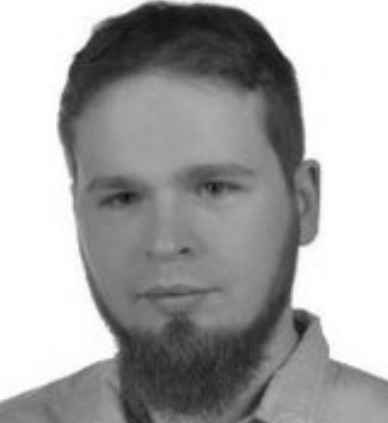
\includegraphics[width=1in,height=1.25in,clip,keepaspectratio]{jjjurec}}]{Jan Jakub Jurec} jest po raz trzeci studentem trzeciego roku Politechniki Wrocławskiej wydziału Elektroniki kierunku Informatyka. Marzeniem autora jest zdanie kursu Organizacja i Architektura Komputerów za trzecim podejściem, jako że kieruje się zasadą "do trzech razy sztuka"! \\
E-mail: jurec@protonmail.com
\end{IEEEbiography}


\begin{IEEEbiography}[{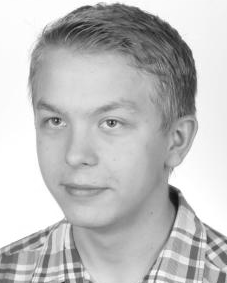
\includegraphics[width=1in,height=1.25in,clip,keepaspectratio]{ftorun}}]{Filip Torun}
jest studentem Politechniki Wrocławskiej wydziału Elektroniki kierunku Informatyka. \\
E-mail: 209428@student.pwr.edu.pl
TODO: MAKE IT PERSONAL
\end{IEEEbiography}

\vfill

\end{document}


